\documentclass[12pt]{article}

\usepackage{co454}

\newcommand{\includelecture}[1]{
  \includepdf[pages=1, pagecommand={\thispagestyle{plain}\section{Lecture {#1}}}]{sections/lec#1.pdf}
  \includepdf[pages=2-, pagecommand=\thispagestyle{plain}]{sections/lec#1.pdf}
  \clearpage
}

\begin{document}

\begin{titlepage}
  \centering
  \vspace*{2in}
  {\huge CO454 - Scheduling Theory}\par
  {\Large (Notes Scans)}\par
  \vspace{0.3in}
  {\large University of Waterloo}\par
  {\large Nicholas Pun}\par
  {\large Spring 2018}\par 
\end{titlepage}
 
\tableofcontents
\clearpage

\section*{Summary}
\addcontentsline{toc}{section}{Summary}
Sections 1 to 8 - See Section Headings (Note: For Section 8, apparently I didn't trust one of the proofs, I've included the offending proof somewhere near the end of the section)

\textit{I usually take notes on loose leaf in-class and then copy them into a dedicated notebook (with some colour-coding and rewording and whatnots) after the class.
I guess I never got around to copying a good chunk of the notes, so below are just raw lecture notes.}

\textit{In case it matters, the colour coding is as follows: Red for theorems, propositions, lemmas, etc., Black for definitions, Blue for generic descriptions}

Lecture 16 - $P||\sum_{C_j}$, $R||\sum_{C_j}$ 

Lecture 17 - $R|\mathrm{pmtn}|C_{\max}$, $O|\mathrm{pmtn}|C_{\max}$

Lecture 18 - Finishing off $O|\mathrm{pmtn}|C_{\max}$, Travelling Salesman Problem

Lecture 19 - Travelling Salesman Problem, Christofides Algorithm

Lecture 20 - $R||C_{\max}$

Lecture 21 - $R||C_{\max}$, Shop Scheduling, Flow  Shop

Lecture 22 - $F2||C_{\max}$

Lecture 23 - $F||C_{\max}$

Lecture 24 - Sevast'janov-Steinitz Lemma (Steinitz lemma in coordinate form)

The main reference was \textit{Scheduling: Theory, Algorithms, and Systems} by Pinedo.
.
\clearpage

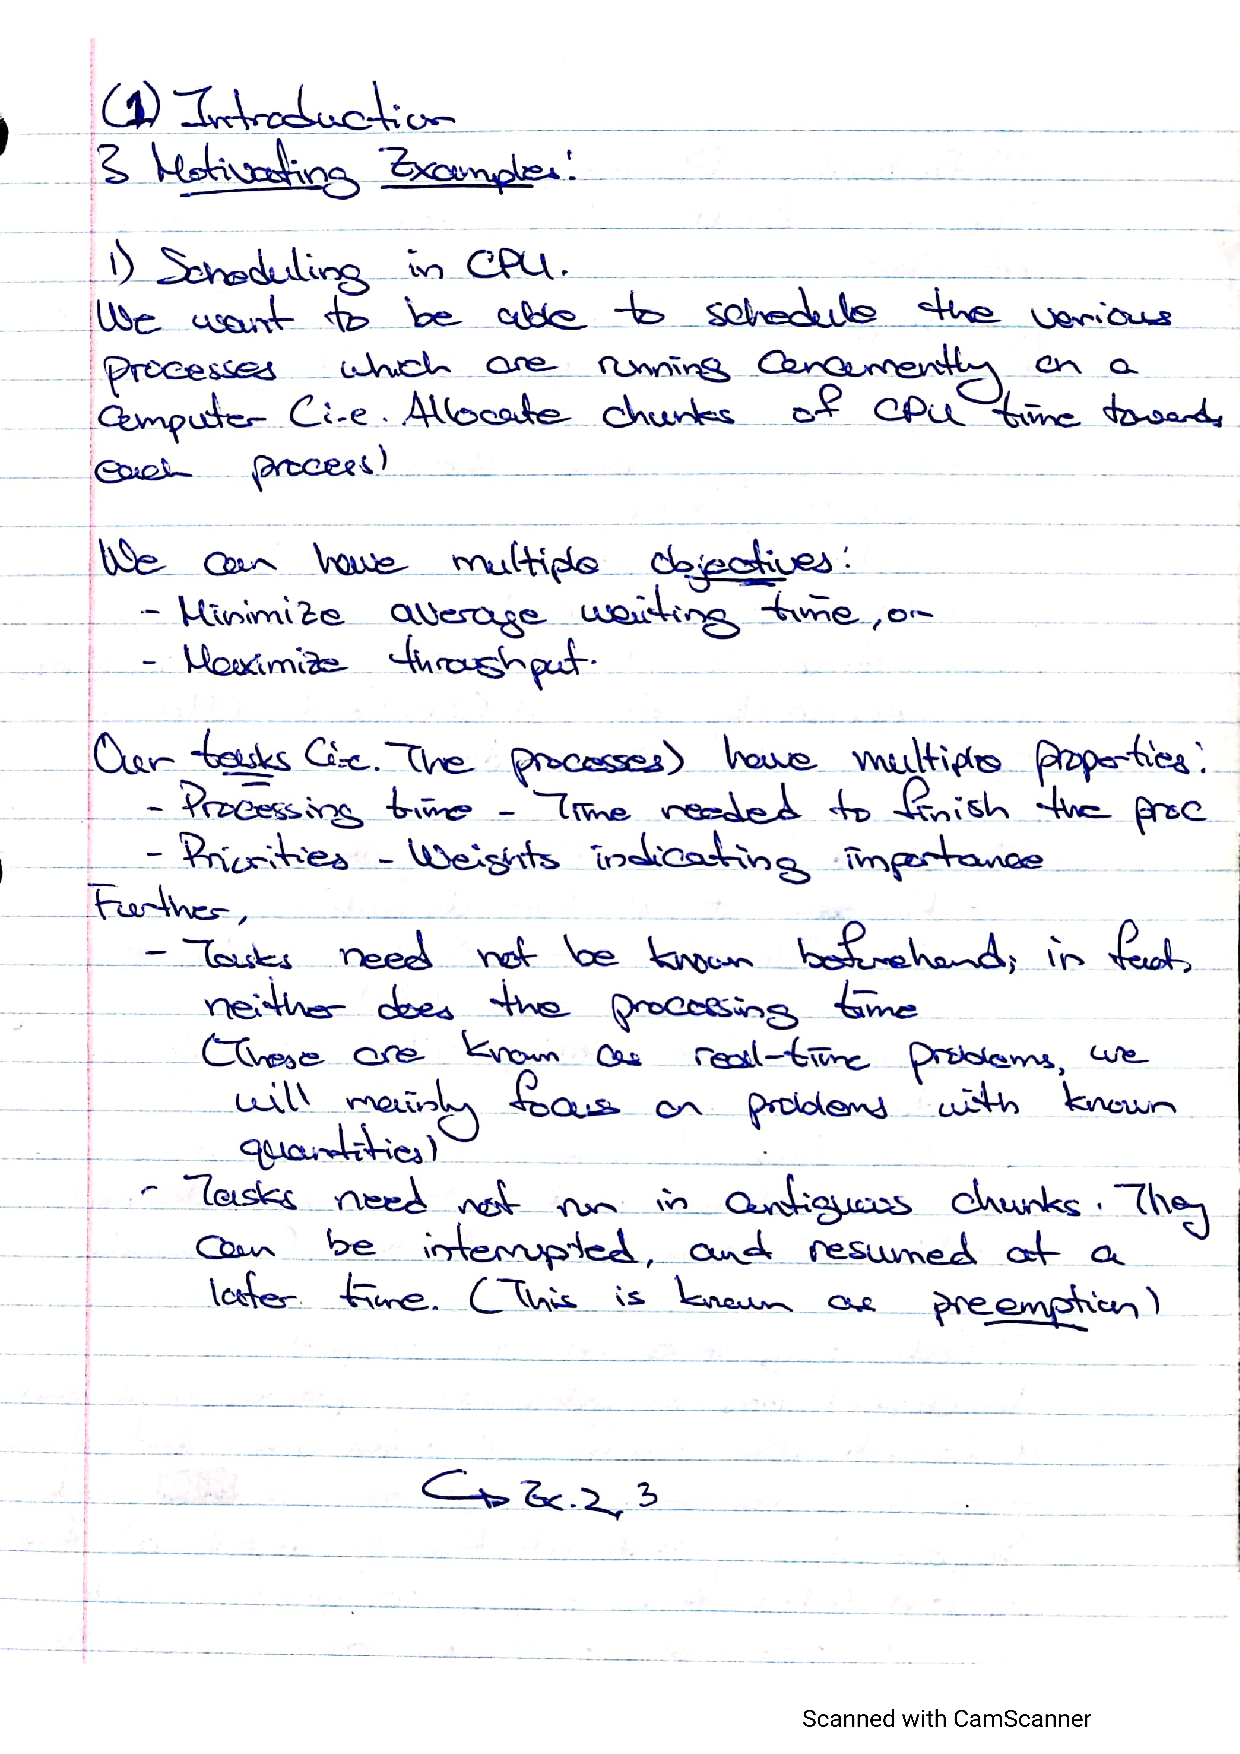
\includepdf[pages=1, pagecommand={\thispagestyle{plain}\section{Introduction}}]{sections/sec1.pdf}
\includepdf[pages=2-, pagecommand=\thispagestyle{plain}]{sections/sec1.pdf}
\clearpage

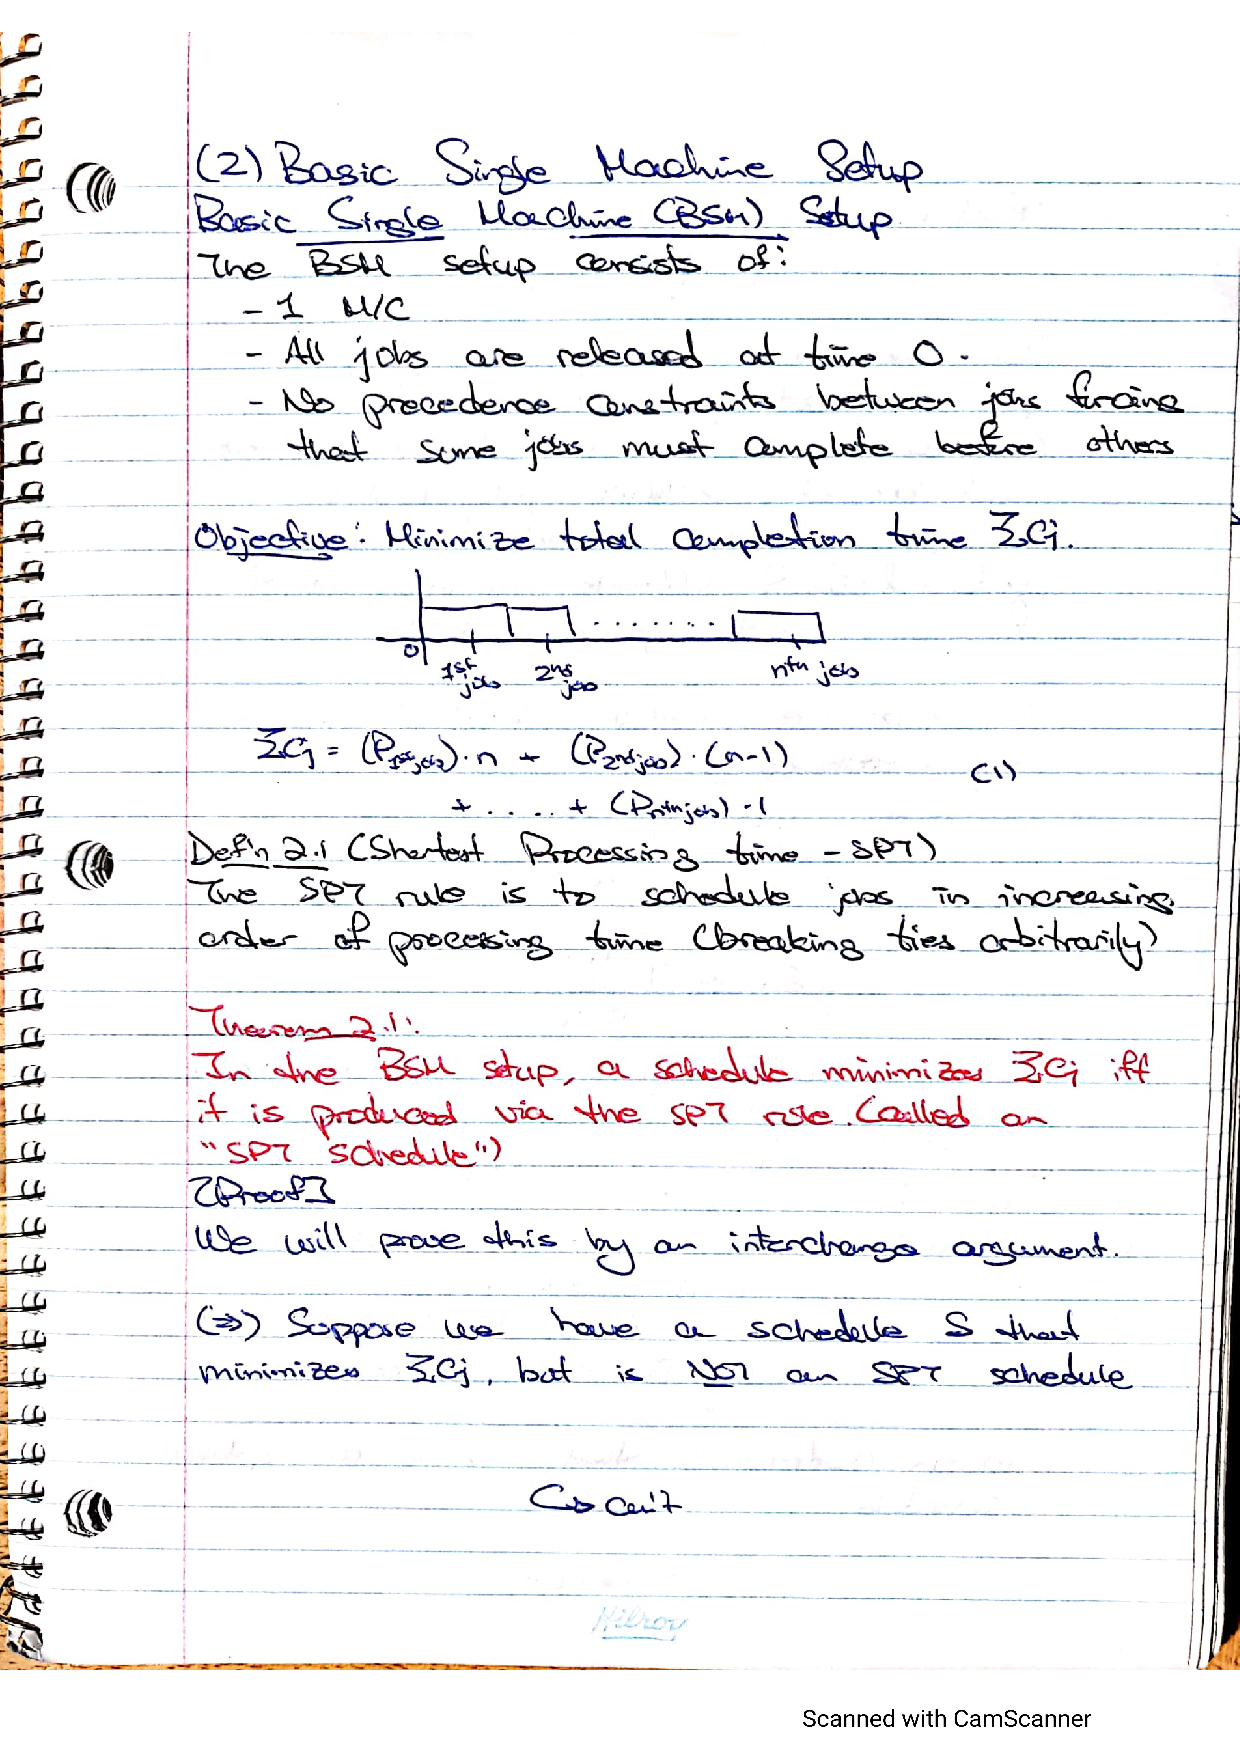
\includepdf[pages=1, pagecommand={\thispagestyle{plain}\section{Basic Single Machine Setup}}]{sections/sec2.pdf}
\includepdf[pages=2-, pagecommand=\thispagestyle{plain}]{sections/sec2.pdf}
\clearpage

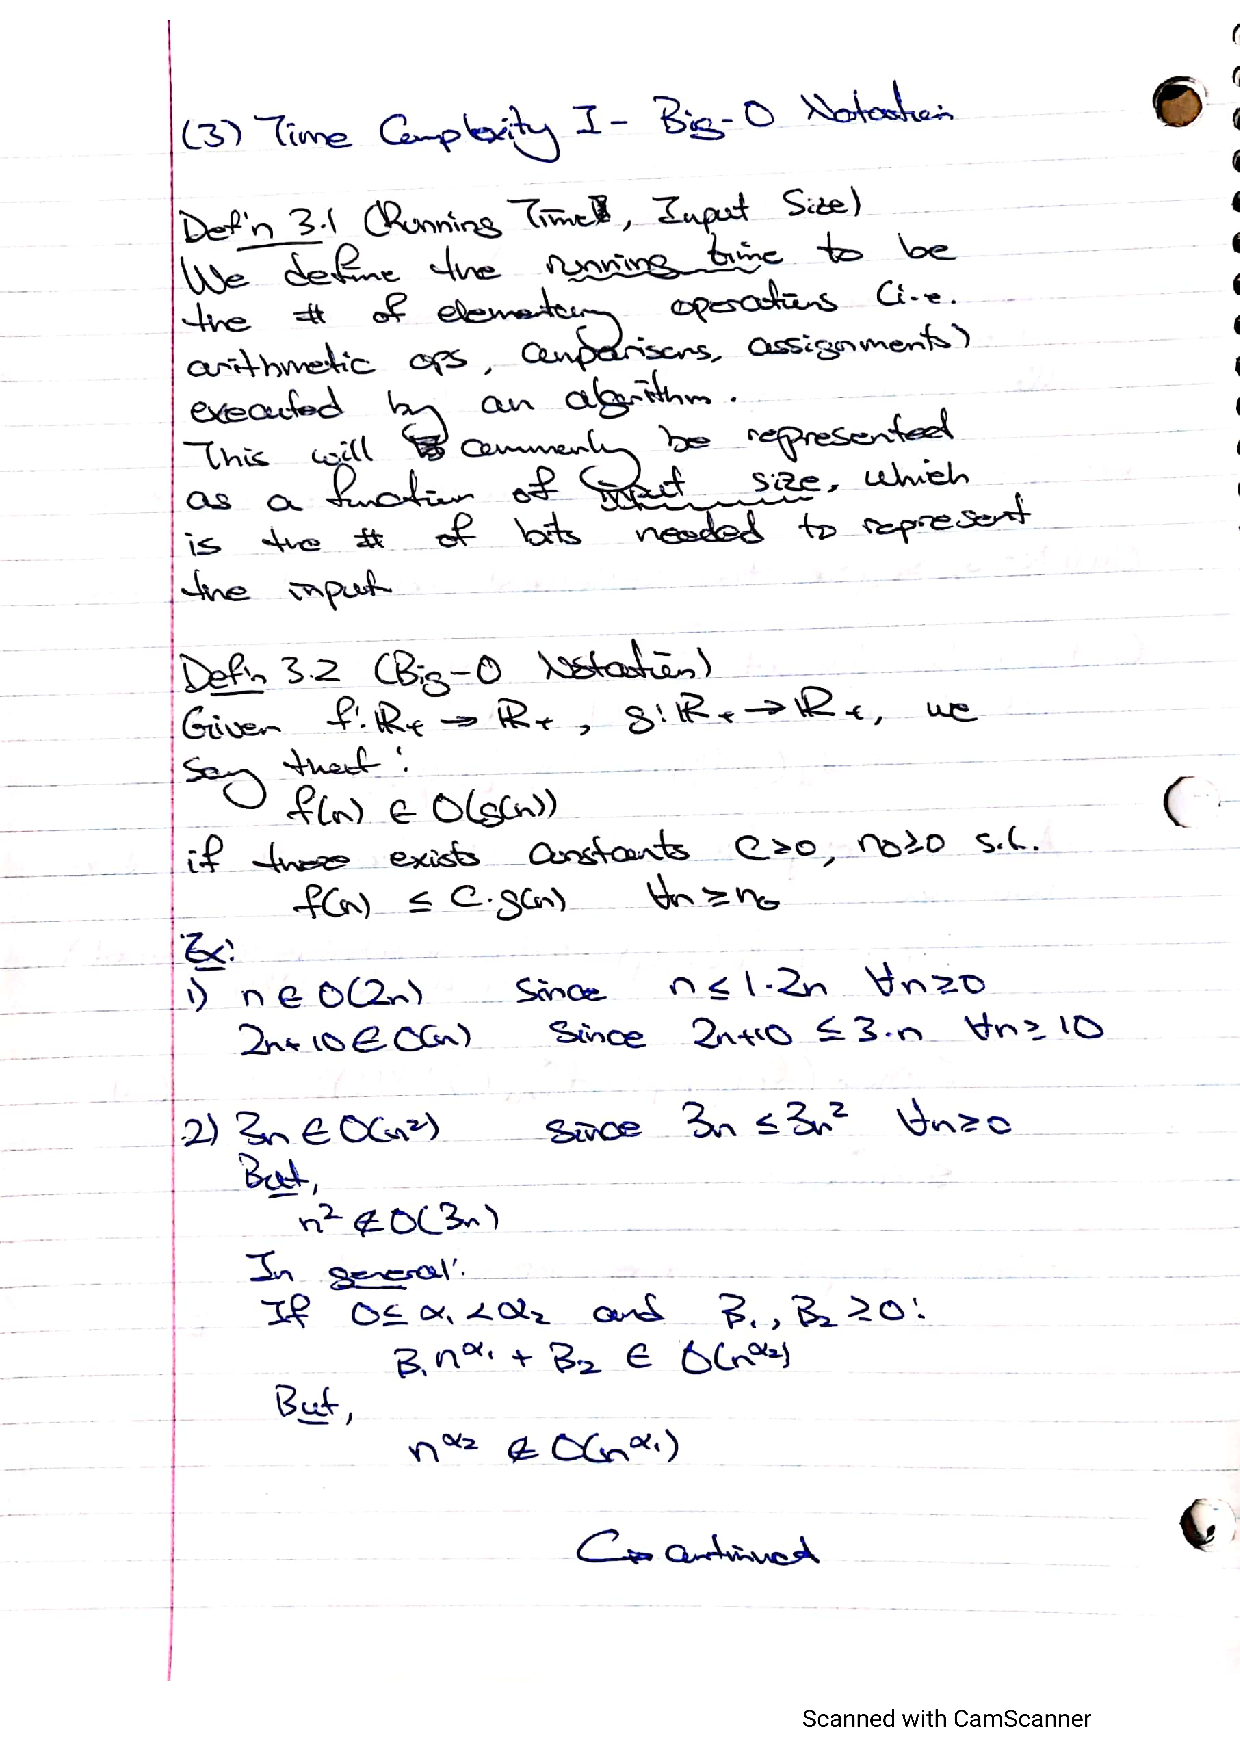
\includepdf[pages=1, pagecommand={\thispagestyle{plain}\section{Time Complexity - Big-O Notation}}]{sections/sec3.pdf}
\includepdf[pages=2-, pagecommand=\thispagestyle{plain}]{sections/sec3.pdf}
\clearpage

\includepdf[pages=1, pagecommand={\thispagestyle{plain}\section{Approximation Algorithms}}]{sections/sec4.pdf}
\includepdf[pages=2-, pagecommand=\thispagestyle{plain}]{sections/sec4.pdf}
\clearpage

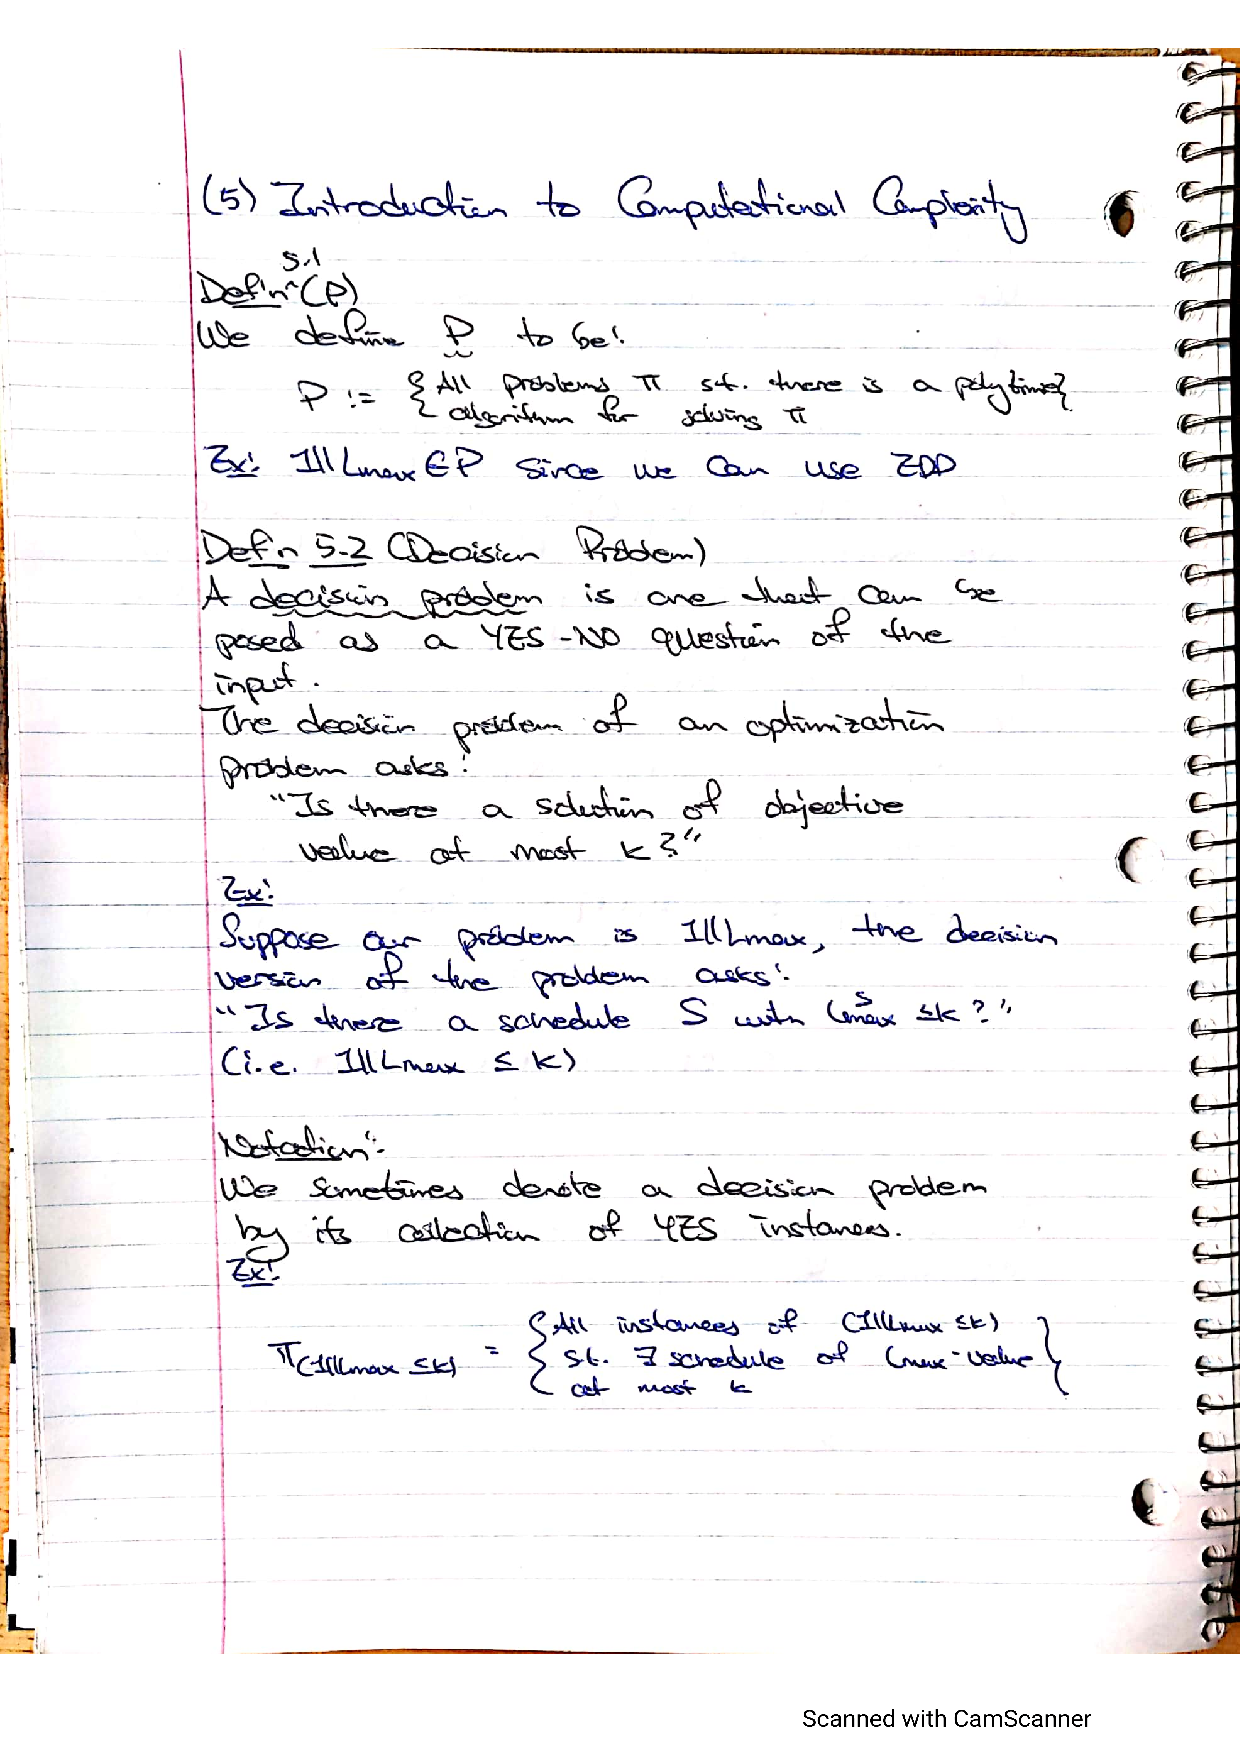
\includepdf[pages=1, pagecommand={\thispagestyle{plain}\section{Basic Computational Complexity}}]{sections/sec5.pdf}
\includepdf[pages=2-, pagecommand=\thispagestyle{plain}]{sections/sec5.pdf}
\clearpage

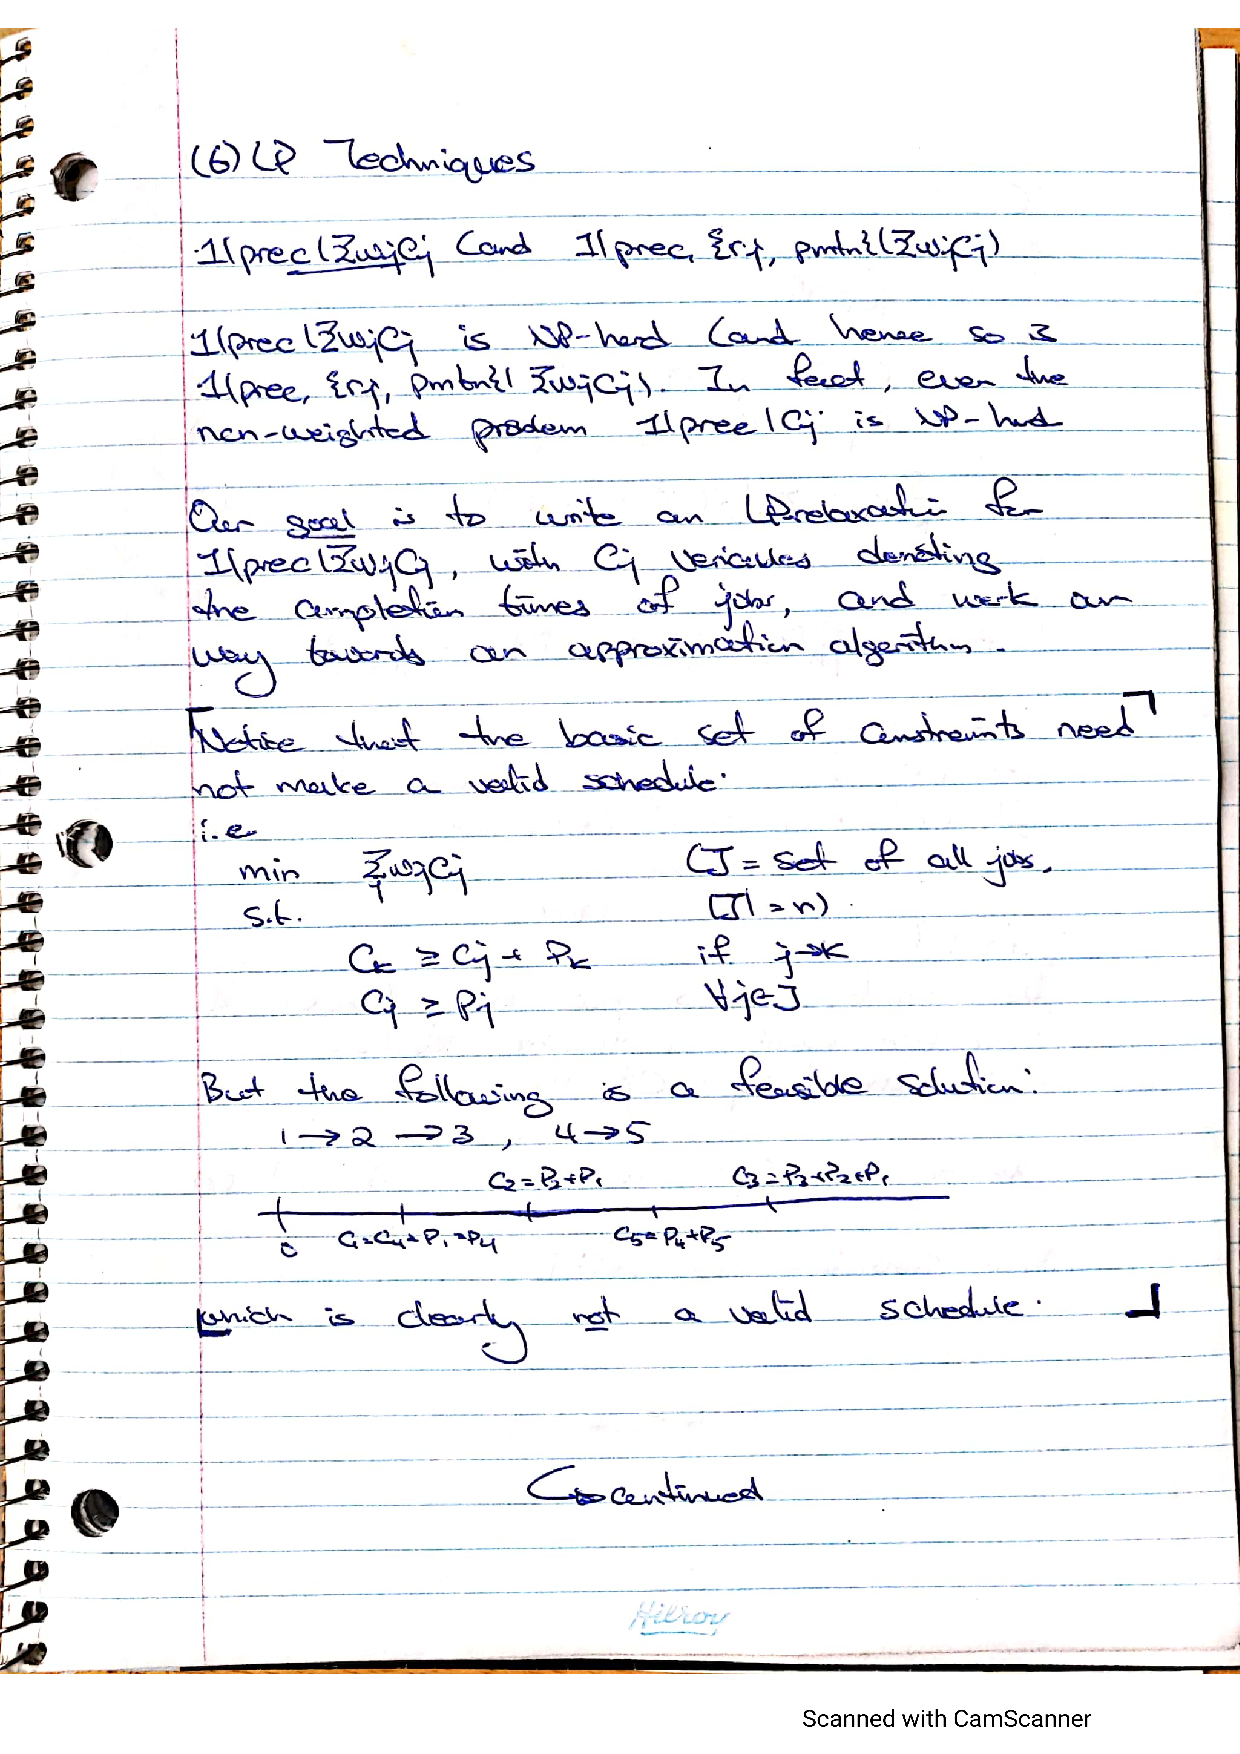
\includepdf[pages=1, pagecommand={\thispagestyle{plain}\section{LP Techniques}}]{sections/sec6.pdf}
\includepdf[pages=2-, pagecommand=\thispagestyle{plain}]{sections/sec6.pdf}
\clearpage

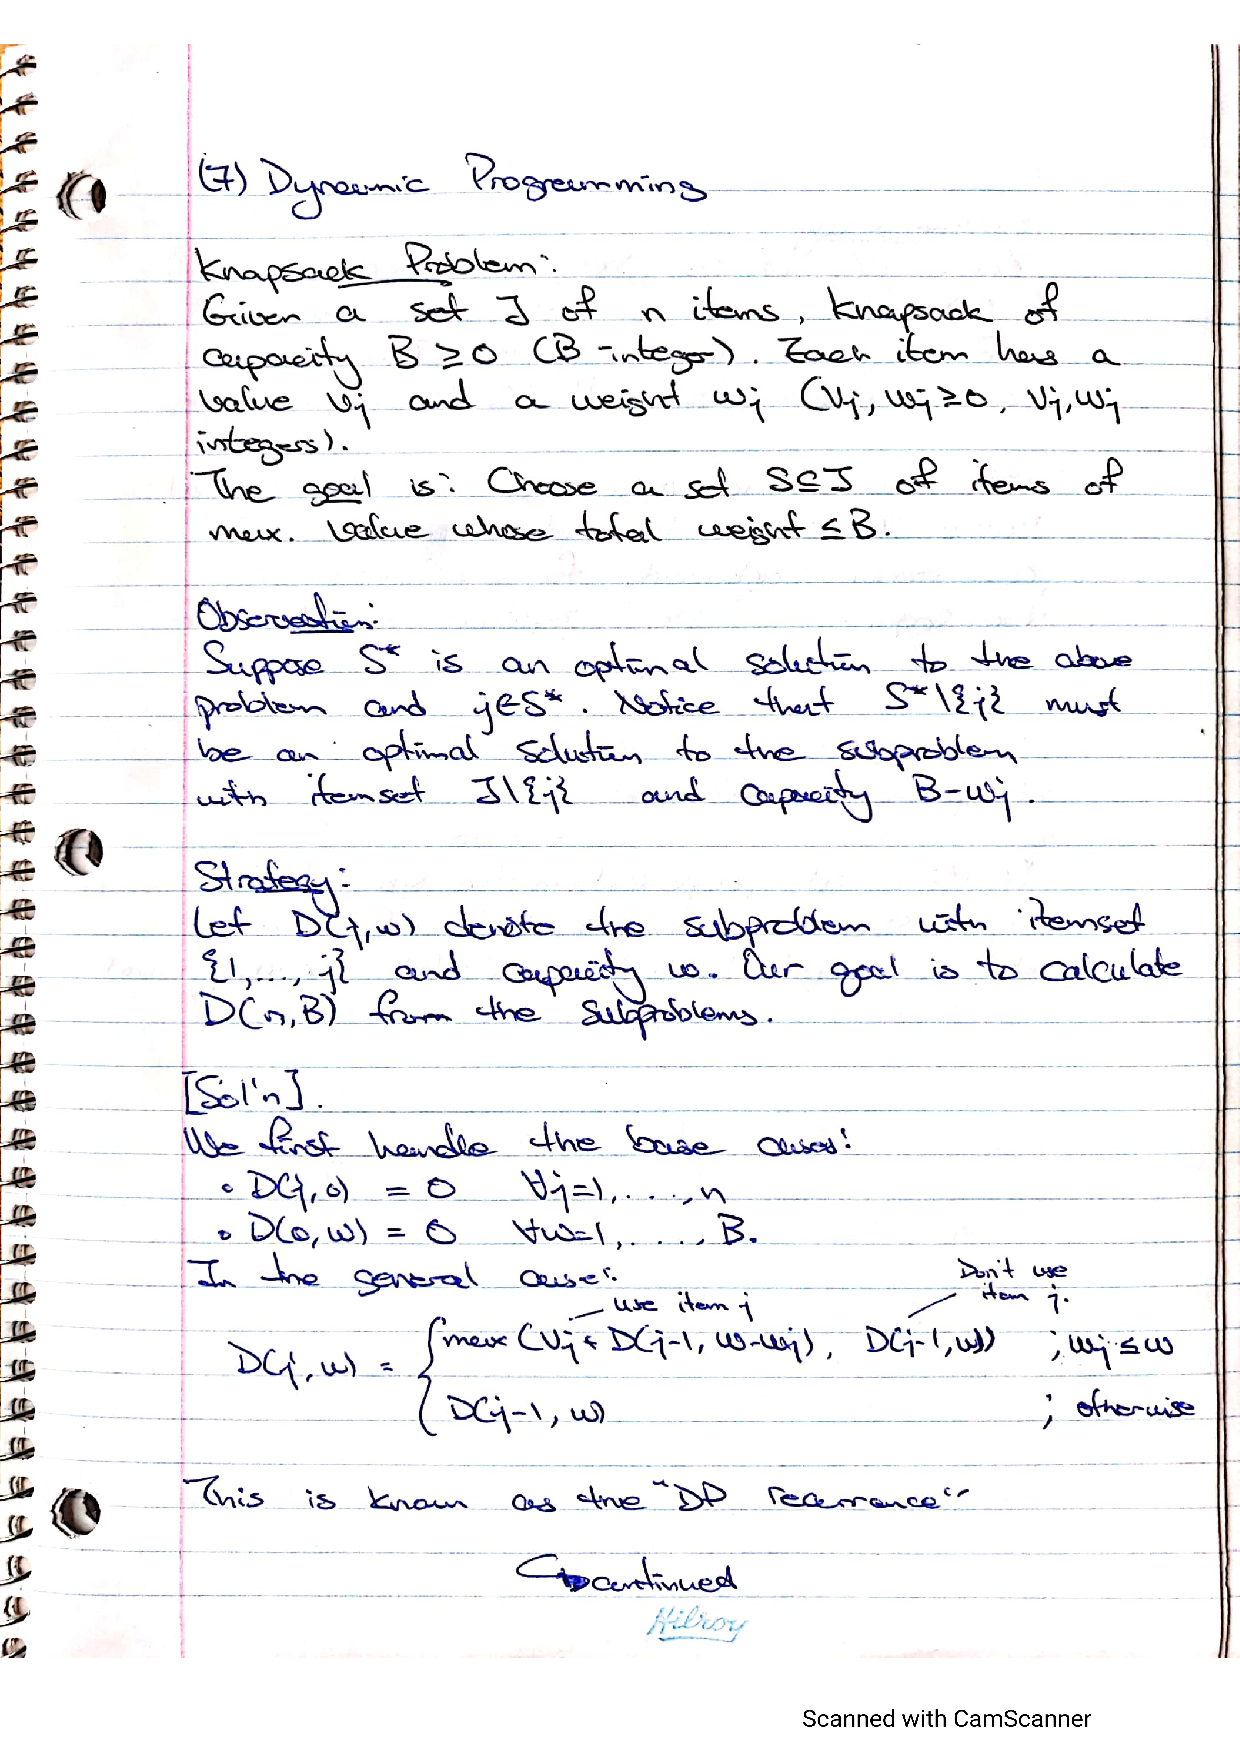
\includepdf[pages=1, pagecommand={\thispagestyle{plain}\section{Dynamic Programming}}]{sections/sec7.pdf}
\includepdf[pages=2-, pagecommand=\thispagestyle{plain}]{sections/sec7.pdf}
\clearpage

\includepdf[pages=1, pagecommand={\thispagestyle{plain}\section{Multiple Machine Models}}]{sections/sec8.pdf}
\includepdf[pages=2-, pagecommand=\thispagestyle{plain}]{sections/sec8.pdf}
\clearpage

\newcount\lecNum
\lecNum=16
\loop
  \includelecture{\the\lecNum}
  \advance \lecNum +1
\ifnum \lecNum<25
\repeat


\end{document}
